\chapter{Transport layer}
\section{UDP (User Data protocol)}
This User Datagram  Protocol  (UDP)  is  defined  to  make  available  a
datagram   mode  of  packet-switched   computer   communication  in  the
environment  of  an  interconnected  set  of  computer  networks\cite{RFC768}. This protocol  provides  a procedure  for application  programs  to send
messages  to other programs  with a minimum  of protocol mechanism.\\
The protocol  is transaction oriented, and delivery and duplicate protection
are not guaranteed.  Applications requiring ordered reliable delivery of
streams of data should use the Transmission Control Protocol (TCP).
\subsection{UDP packet format}
\begin{figure}[h]
\centering\footnotesize
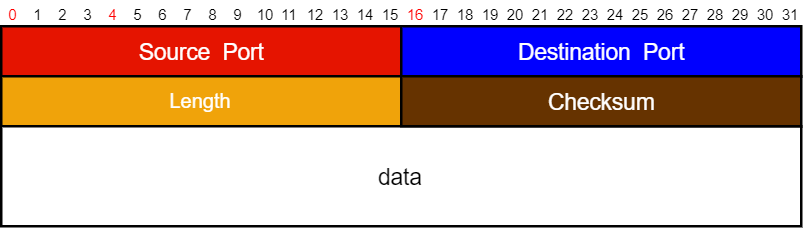
\includegraphics[scale=0.5]{Images/Transport/UDP_packet_format}
\caption{UDP packet format.}
\end{figure}
\begin{itemize}
\item{\textbf{Source Port (}16 bits\textbf{)}\\
The source port number}
\item{\textbf{Destination Port (}16 bits\textbf{)}\\
The destination port number}
\item{\textbf{Length (16 bits)}
The length in octets of this user datagram including this header and the data}
\item{\textbf{Checksum (}16 bits\textbf{)}\\
The checksum of information from the IP header, the UDP header, and the data, padded with zero octets at the end (if necessary) to make a multiple of two octets.\\
The pseudo header, conceptually prefixed to the UDP header, contains the source  address,  the destination  address,  the protocol,  and the  UDP length.   This information gives protection against misrouted datagrams. This checksum procedure is the same as is used in TCP.\\
If the computed checksum is zero, it is transmitted as all ones (the equivalent in one's complement arithmetic). An all zero transmitted
checksum value means that the transmitter generated no checksum (for debugging or for higher level protocols that don't care).
\begin{figure}[H]
\centering\footnotesize
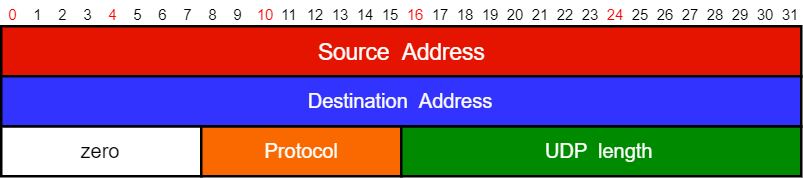
\includegraphics[scale=0.5]{Images/Transport/UDP_pseudo_header}
\caption{Pseudo header.}
\end{figure}
}
\end{itemize}

\section{TCP (Transmission Control protocol)}
The Transmission Control Protocol (TCP) is intended for use as a highly
reliable host-to-host protocol between hosts in packet-switched computer
communication networks, and in interconnected systems of such networks\cite{RFC793}.
\subsection{TCP packet format}
\begin{figure}[h]
\centering\footnotesize
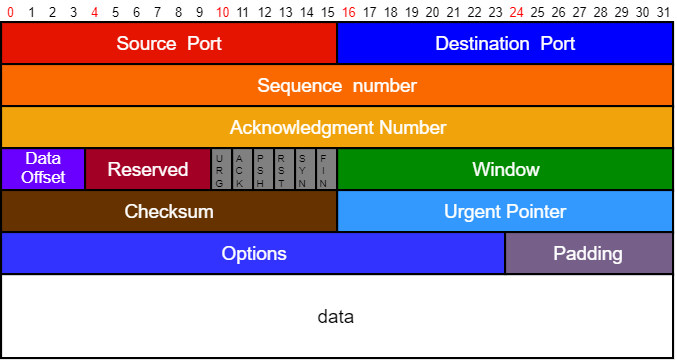
\includegraphics[scale=0.6]{Images/Transport/TCP_packet_format}
\caption{TCP packet format.}
\end{figure}

\begin{itemize}
\item{\textbf{Source Port (}16 bits\textbf{)}\\
The source port number}
\item{\textbf{Destination Port (}16 bits\textbf{)}\\
The destination port number}
\item{\textbf{Sequence Number (}32 bits\textbf{)}\\
The sequence number of the first data octet in this segment (except when SYN is present). If SYN is present the sequence number is the initial sequence number (ISN) and the first data octet is ISN+1.}
\item{\textbf{Acknowledgment Number (}32 bits\textbf{)}\\
If the ACK control bit is set this field contains the value of the next sequence number the sender of the segment is expecting to receive. Once a connection is established this is always sent.}
\item{\textbf{Data Offset (}4 bits\textbf{)}\\
The number of 32 bit words in the TCP Header.  This indicates where the data begins.  The TCP header (even one including options) is an integral number of 32 bits long.}
\item{\textbf{Reserved (}6 bits\textbf{)}\\
Reserved for future use.  Must be zero.}
\item{\textbf{Control Bits  (}6 bits (from left to right)\textbf{)}\\
\begin{table}[h]
\centering\footnotesize
\begin{tabular}{rl}
\multicolumn{1}{c}{\textbf{Bit}} & \multicolumn{1}{c}{\textbf{Meaning}}\\
\hline
\textbf{URG} & Urgent Pointer field significant\\
\textbf{ACK} & Acknowledgment field significant\\
\textbf{PSH} & Push Function\\
\textbf{RST} & Reset the connection\\
\textbf{SYN} & Synchronize sequence numbers\\
\textbf{FIN} & No more data from sender
\end{tabular}
\end{table}
}
\item{\textbf{Window (}6 bits\textbf{)}\\
The number of data octets beginning with the one indicated in the acknowledgment field which the sender of this segment is willing to accept.}
\item{\textbf{Checksum (}16 bits\textbf{)}\\
The checksum field is the 16 bit one's complement of the one's complement sum of all 16 bit words in the header and text.  If a segment contains an odd number of header and text octets to be checksummed, the last octet is padded on the right with zeros to form a 16 bit word for checksum purposes.\\
The pad is not transmitted as part of the segment.  While computing the checksum, the checksum field itself is replaced with zeros. The checksum also covers a 96 bit pseudo header conceptually prefixed to the TCP header.\\
This pseudo header contains the Source Address, the Destination Address, the Protocol, and TCP length. This gives the TCP protection against misrouted segments.  This information is carried in the Internet Protocol and is transferred across the TCP/Network interface in the arguments or results of calls by the TCP on the IP.\\
\begin{figure}[H]
\centering\footnotesize
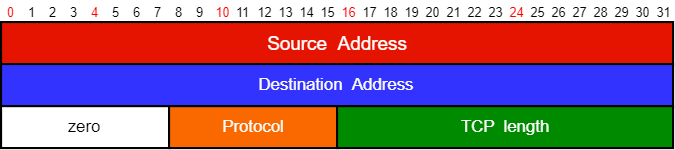
\includegraphics[scale=0.6]{Images/Transport/TCP_pseudo_header}
\caption{Pseudo header.}
\end{figure}
The TCP Length is the TCP header length plus the data length in octets (this is not an explicitly transmitted quantity, but is computed), and it does not count the 12 octets of the pseudo header.}
\item{\textbf{Urgent Pointer (}16 bits\textbf{)}\\
This field communicates the current value of the urgent pointer as a positive offset from the sequence number in this segment.  The urgent pointer points to the sequence number of the octet following the urgent data.  This field is only be interpreted in segments with the URG control bit set.}
\item{\textbf{Options (}variable length\textbf{)}\\
Options may occupy space at the end of the TCP header and are a multiple of 8 bits in length. All options are included in the checksum. An option may begin on any octet boundary. There are two cases for the format of an option:
\begin{itemize}
\item{\textbf{Case 1:}\\
A single octet of option-kind.}
\item{\textbf{Case 2:}\\
An octet of option-kind, an octet of option-length, and the actual option-data octets.}
\end{itemize}
The option-length counts the two octets of option-kind and option-length as well as the option-data octets. Note that the list of options may be shorter than the data offset field might imply.\\
The content of the header beyond the End-of-Option option must be header padding (i.e., zero). A TCP must implement all options.\\
Currently defined options include (kind indicated in octal):
\begin{table}[h]
\centering \footnotesize
\begin{tabular}{ccl}
\textbf{Kind} & \textbf{Length} & \textbf{Meaning}\\
\hline
\textit{0} & \textit{-} & End of option list\\
\textit{1} & \textit{-} & No-Operation\\
\textit{2} & \textit{4} & Maximum Segment Size
\end{tabular}
\end{table}       
}
\item{\textbf{Padding (}variable length\textbf{)}\\
The TCP header padding is used to ensure that the TCP header ends and data begins on a 32 bit boundary. The padding is composed of zeros.}
\end{itemize}

\vspace{15cm}
\subsection{Connection state diagram}
A connection progresses through a series of states during its lifetime, that are (Figure \ref{connection_state}):
\begin{itemize}
\item{\textbf{LISTEN}\\
waiting for a connection request from any remote TCP and port.}
\item{\textbf{SYN-SENT}\\
waiting for a matching connection request after having sent a connection request.}
\item{\textbf{SYN-RECEIVED}\\
waiting for a confirming connection request acknowledgment after having both received and sent a connection request.}
\item{\textbf{ESTABLISHED}\\
an open connection in which data received can be delivered to the user.  The normal state for the data transfer phase of the connection.
\item{\textbf{FIN-WAIT-1}\\
waiting for a connection termination request from the remote TCP, or an acknowledgment of the connection termination request previously sent.}
\item{\textbf{FIN-WAIT-2}\\
waiting for a connection termination request from the remote TCP.}
\item{\textbf{CLOSE-WAIT}}\\
waiting for a connection termination request from the local user.}
\item{\textbf{CLOSING}\\
waiting for a connection termination request acknowledgment from the remote TCP.}
\item{\textbf{LAST-ACK}\\
waiting for an acknowledgment of the connection termination request previously sent to the remote TCP (which includes an acknowledgment of its connection termination request).}
\item{\textbf{TIME-WAIT}\\
waiting for enough time to pass to be sure the remote TCP received the acknowledgment of its connection termination request.}
\item{\textbf{CLOSED}\\
fictional state that represents no connection state at all.}
\end{itemize}

In connection state diagram, each transition shows the event that generates the transition and the operation done as response to the event (Figure \ref{transition}). Hence the event can be seen like the event for which a callback will be called and the operation is the set of instructions implemented in the code of the callback. The response x indicates that no action is performed.\\

\begin{figure}[H]
\centering\footnotesize
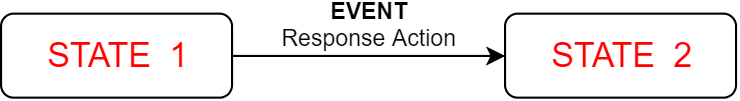
\includegraphics[scale=0.3]{Images/Transport/transition}
\caption{Example of transition.}\label{transition}
\end{figure}

\begin{figure}[H]
\centering\footnotesize
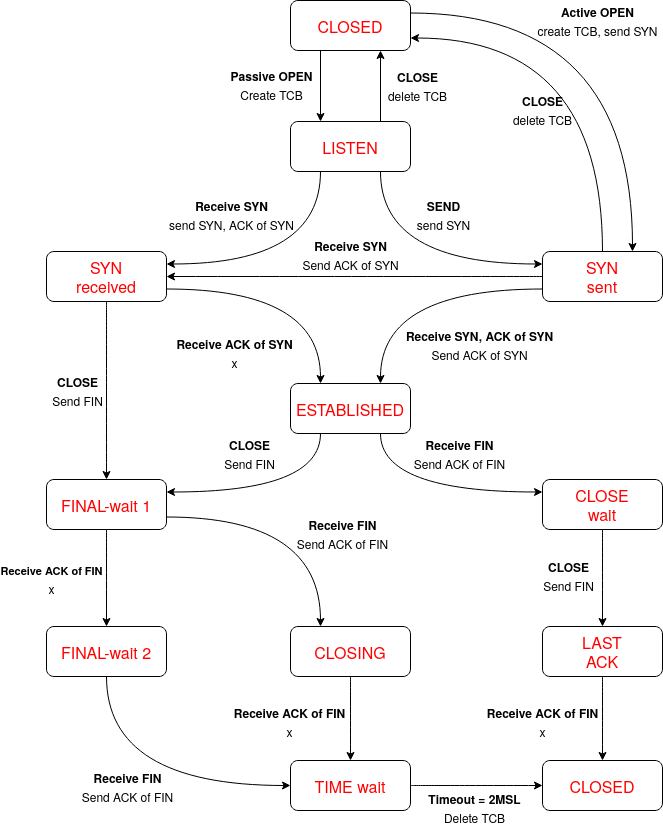
\includegraphics[scale=0.58]{Images/Transport/finite_state}
\caption{Connection state diagram.}\label{connection_state}
\end{figure}
\vspace{2cm}
\subsection{Management packet loss}
The warranty of the delivery of a packet was implemented at lower level. At layer 4, to understand if the packet is arrived to the receiver, the sender receives a packet called Acknowledgment (ACK).\\
When the sender sends a packet, he waits for a while. During this period, the sender is almost sure that ACK has to arrive. If it doesn't receive the ACK in this period, it sends again the same packet to the receiver. This behaviour is essential in implementation of sender code to receive a loss (Figure \ref{timeout}).\\

\begin{figure}[H]
\centering\footnotesize
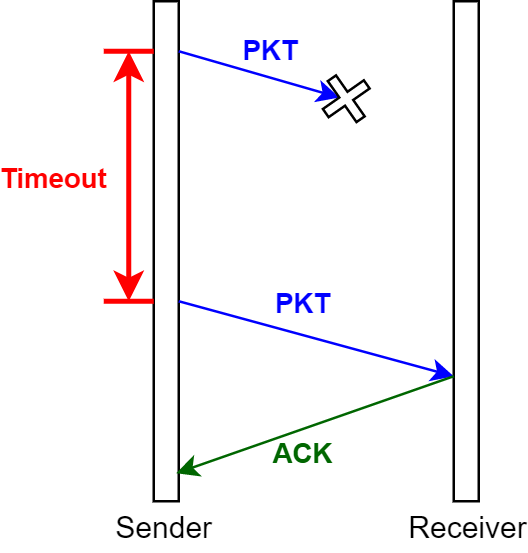
\includegraphics[scale=0.4]{Images/Transport/timeout}
\caption{Timeout for waiting time of ACK.}\label{timeout}
\end{figure}

If a loss of the ack occurs, the receiver must be able to handle the duplicate packet. Hence the packets need to have an indentifier that allows the receiver to  be aware that packet is the same of the first one (Figure \ref{loss_ACK}).\\

\begin{figure}[H]
\centering\footnotesize
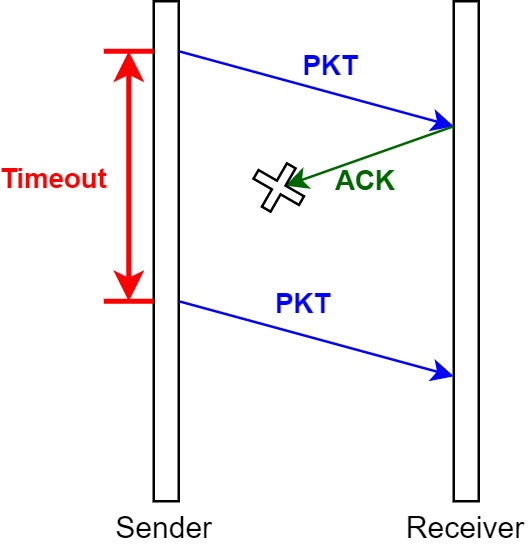
\includegraphics[scale=0.4]{Images/Transport/loss_ACK}
\caption{Management by receiver of doubled packets.}\label{loss_ACK}
\end{figure}

If the ACks arrive with a certain delay, we need to enumerate them. The reason can be found looking to Figure \ref{delay_ACK}. If the sender sends a packet \textbf{PKT 1} and waits for its ACK for a timeout w. If the corresponding ACK arrives after w seconds, the sender has already resent \textbf{PKT 1} thinking that it's been lost.\\
Then suppose that the sender receives \textbf{ACK of first PKT 1}, so it sends the next packet \textbf{PKT 2} but this will be lost. After a while the sender receives the \textbf{ACK of second PKT 1} but, if ACKs are not identified by numbers, the sender can think that the ACK is relative to \textbf{PKT 2} because it already receives \textbf{ACK of PKT 1}.\\

\begin{figure}[H]
\centering\footnotesize
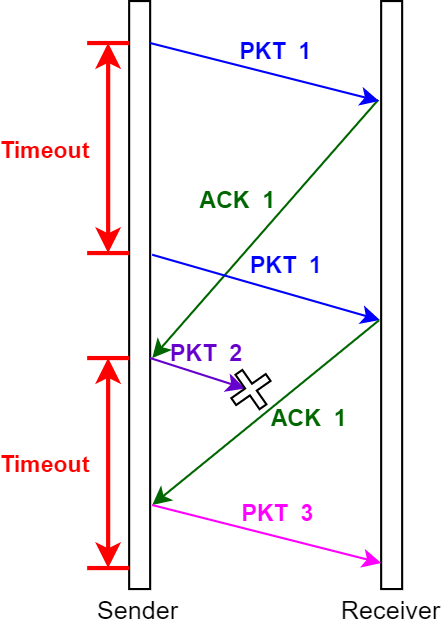
\includegraphics[scale=0.4]{Images/Transport/delay_ACK}
\caption{Problem with delayed ACK.}\label{delay_ACK}
\end{figure}

During the latency, sending a packet and waiting for its ACK before sending the new one causes waste of time and bandwidth capacibity (Figure \ref{waste_time}.\\

\begin{figure}[H]
\centering\footnotesize
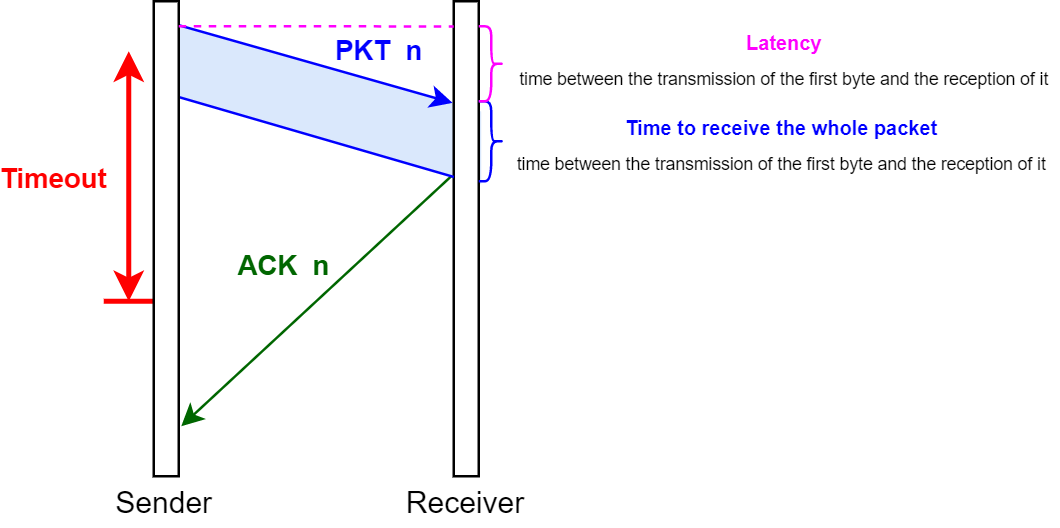
\includegraphics[scale=0.4]{Images/Transport/waste_time}
\caption{Transmission of a packet.}\label{waste_time}
\end{figure}

We send in optimistic way more packets to fit the network capacity (pipeline), betting that the whole packet will arrive to destination. The latency becomes negletable with respect to the time needed to send all the packets.

\subsection{Segmentation of the stream}
The buffer is split into segments of bytes and the numbers identify the byte positions. The identifier of the packet is the offset of the stream.\\
The \textbf{sequence number} is the position(offset of the first byte in the segment. The ACK number is the first empty (not yet received) position in the stream (e.g. in Figure \ref{segmentation} if segment 1, segment 2 and segment 4 have been received all the ACK number is 21).\\

\begin{figure}[H]
\centering\footnotesize
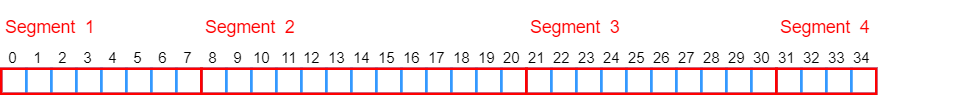
\includegraphics[scale=0.5]{Images/Transport/segmentation}
\caption{Example of segmentation of the stream.}\label{segmentation}
\end{figure}

\subsection{Automatic Repeat-reQuest (ARQ)}
ARQ is a control strategy of the errors that detects an error (without correction). Corrupted packets are discarded and there is the request of their retransmissions.
\begin{sidewaystable}
\footnotesize\centering
\begin{tabular}{|llllllll|}
\multicolumn{1}{l}{\textbf{TX BUF}} & \textbf{RX BUF} & \textbf{NAME} & \textbf{packet id} & \textbf{Timeout} & \textbf{Sender}  & \textbf{Receiver actions} & \multicolumn{1}{l}{\textbf{Ack type}}\\
\hline
{1} & {1} & {Stop \& Wait} & {1-bit} & {single} & {Send a packet awaits reply with the} & {Respond ACK with packet id.} & {single ACK}\\
& & & & & {same id, after timeout send packet id} & & \\
\hline
N & 1 & {go-back-N} & {log Nbit} & {window} & {Send N packets after start ptr.} & {Replies ACK with id only if} & {cumulative ack}\\
& & & & & {Awaits reply with id. ptr = id} & {id is old id + 1} &\\
\hline
{N} & {N} & {Selective Repeat} & {log Nbit} & {Single for} & {Send N packets after the last ACK.} & {ACK replies to each packet with} & {selective ack}\\
& & & & & {Each ACK is specific to each packet,} & {the id of the packet falling} & \\
& & & & {each frame} & {each packet has its own timeout.} & {in the receiving window.} & \\
& & & & & {The sliding window proceeds from the} & {} &\\
& & & & & {most recent packet received without} & {} &\\
& & & & & {previous "holes".} & {} &\\
\hline
N & N & {Sliding window} & {log Nbit} & {window} & {Send N packets after start ptr.} & {Answers ACK cumulative} & {ACK}\\
& & {(TCP)} & & & {Each window has its timeout if it is} & {} & \\
& & & & & {not set (as soon as it is updated)} & &\\
& & & & & {it is set from the first sending.} & &\\
& & & & & {The sliding window resets to the} & &\\
& & & & & {cumulative attack.} & &\\
\hline
N & N  & {Sliding window} & {log Nbit} & {Single for} & {Send N packets after ptr start.} & {Responds to ACK +} & {cumulative ACK}\\
& & {(TCP) + SACK}& & & {Each ack is cumulative.} & {Contiguous data blocks} & {+ SACK}\\
& & & & {each frame} & {Each packet has its own timeout.} & &\\
& & & & & {The sliding window resets itself} & &\\
& & & & & {to the cumulative packet} & &\\
\hline
\end{tabular}
\end{sidewaystable}
\vspace{13cm}
\subsection{TCP window}
A variable window size is usually used and it's increased when there is no packet loss. Variable timeouts are used also in this system. If a packet is lost, the ACK is stopped because it's cumulative and the size of the window is set again to 1.\\
There are two types of control:
\begin{itemize}
\item{\textbf{Flow control}\\
made by receiver}
\item{\textbf{Congestion control}\\
managing packet losses}
\end{itemize}
There is usually a threshold, called \textbf{ssthresh}, and the actual window size is called \textbf{cwnd}. If \textbf{cwnd} is less than \textbf{ssthresh}
the window size will be doubled at next step.\\
After the first increase of the window size up to the double of \textbf{ssthresh}, the window size will increase linearly in the range of \textbf{$\mathtt{[ssthresh, 2*ssthresh]}$}
\begin{figure}[H]
\centering\footnotesize
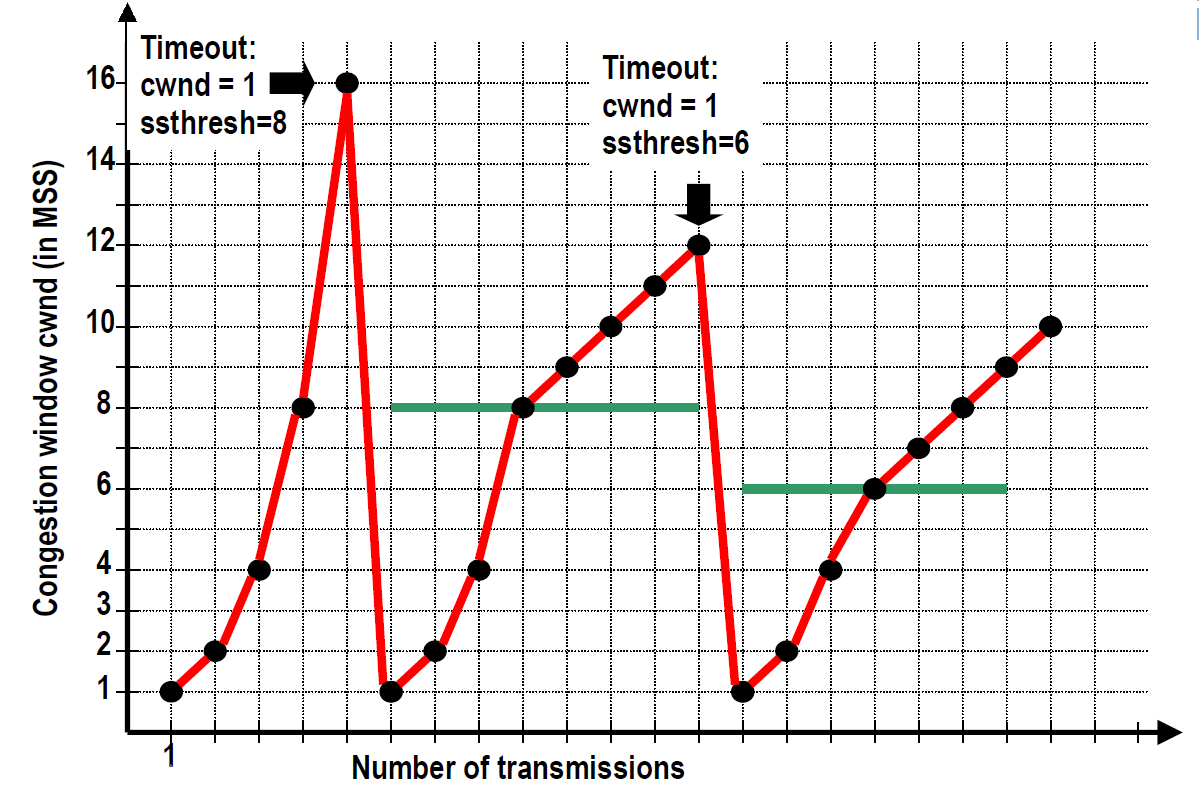
\includegraphics[scale=0.4]{Images/Transport/example_cwnd}
\caption{Example of window size update.}\label{cwnd}
\end{figure}